\documentclass{wissdoc}
% Autor: Roland Bless 1996-2005, bless@tm.uka.de
% ----------------------------------------------------------------
% Diplomarbeit - Hauptdokument
% ----------------------------------------------------------------
%%
%% $Id: diplarb.tex 5 2005-10-10 20:55:48Z bless $
%%
% wissdoc Optionen: draft, relaxed, pdf --> siehe wissdoc.cls
% ------------------------------------------------------------------
% Weitere packages: (Dokumentation dazu durch "latex <package>.dtx")
% \usepackage{varioref}
% \usepackage{verbatim}
% \usepackage{float}    %z.B. \floatstyle{ruled}\restylefloat{figure}
% \usepackage{subfigure}
% \usepackage{color}    % Farbiger/grauer Text
% \usepackage{colortbl}   % Farbige/graue Tabellenzeilen und -spalten!! <--
% \usepackage{fancybox} % f�r schattierte,ovale Boxen etc.
% \usepackage{tabularx} % automatische Spaltenbreite
% \usepackage{supertab} % mehrseitige Tabellen
%% ---------------- end of usepackages -------------

%% Informationen f�r die PDF-Datei
\hypersetup{
 pdfauthor={Christina Pildner},
 pdftitle={Not set}
 pdfsubject={Not set},
 pdfkeywords={Not set}
}

% Macros, nicht unbedingt notwendig
%%%%%%%%%%%%%%%%%%%%%%%%%%%%%%%%%%%%%%%%%%%%%%%%%%%%%%%%%%
% macros.tex -- einige mehr oder weniger nuetzliche Makros
% Autor: Roland Bless 1998
%%%%%%%%%%%%%%%%%%%%%%%%%%%%%%%%%%%%%%%%%%%%%%%%%%%%%%%%%%
% $Id: macros.tex 4 2005-10-10 20:51:21Z bless $
%%%%%%%%%%%%%%%%%%%%%%%%%%%%%%%%%%%%%%%%%%%%%%%%%%%%%%%%%%


%%%%%%%%%%%%%%%%%%%%%%%
% Kommentare 
%%%%%%%%%%%%%%%%%%%%%%%
\ifnotdraftelse{
\newcommand{\Kommentar}[1]{}
}{\newcommand{\Kommentar}[1]{{\em #1}}}
% Alles innerhalb von \Hide{} oder \ignore{} 
% wird von LaTeX komplett ignoriert (wie ein Kommentar)
\newcommand{\Hide}[1]{}
\let\ignore\Hide

%%%%%%%%%%%%%%%%%%%%%%%%%
% Leere Seite ohne Seitennummer, wird aber gezaehlt
%%%%%%%%%%%%%%%%%%%%%%%%%

\newcommand{\leereseite}{% Leerseite ohne Seitennummer, n�chste Seite rechts (wenn 2-seitig)
 \clearpage{\pagestyle{empty}\cleardoublepage}
}

%%%%%%%%%%%%%%%%%%%%%%%%%%
% Neue Seite rechts, leere linke Seite ohne Headings
%%%%%%%%%%%%%%%%%%%%%%%%%%
\newcommand{\xcleardoublepage}
{{\pagestyle{empty}\cleardoublepage}}

%%%%%%%%%%%%%%%%%%%%%%%%%%
% Tabellenspaltentypen (benoetigt colortbl)
%%%%%%%%%%%%%%%%%%%%%%%%%%
\newcommand{\PBS}[1]{\let\temp=\\#1\let\\=\temp}
\newcolumntype{y}{>{\PBS{\raggedright\hspace{0pt}}}p{1.35cm}}
\newcolumntype{z}{>{\PBS{\raggedright\hspace{0pt}}}p{2.5cm}}
\newcolumntype{q}{>{\PBS{\raggedright\hspace{0pt}}}p{6.5cm}}
\newcolumntype{g}{>{\columncolor[gray]{0.8}}c} % Grau
\newcolumntype{G}{>{\columncolor[gray]{0.9}}c} % helleres Grau

%%%%%%%%%%%%%%%%%%%%%%%%%%
% Anf�hrungszeichen oben und unten
%%%%%%%%%%%%%%%%%%%%%%%%%%
\newcommand{\anf}[1]{"`{#1}"'}

%%%%%%%%%%%%%%%%%%%%%%%%%%
% Tiefstellen von Text
%%%%%%%%%%%%%%%%%%%%%%%%%%
% S\tl{0} setzt die 0 unter das S (ohne Mathemodus!)
% zum Hochstellen gibt es uebrigens \textsuperscript
\makeatletter
\DeclareRobustCommand*\textlowerscript[1]{%
  \@textlowerscript{\selectfont#1}}
\def\@textlowerscript#1{%
  {\m@th\ensuremath{_{\mbox{\fontsize\sf@size\z@#1}}}}}
\let\tl\textlowerscript
\let\ts\textsuperscript
\makeatother

%%%%%%%%%%%%%%%%%%%%%%%%%%
% Gau�-Klammern
%%%%%%%%%%%%%%%%%%%%%%%%%%
\newcommand{\ceil}[1]{\lceil{#1}\rceil}
\newcommand{\floor}[1]{\lfloor{#1}\rfloor}

%%%%%%%%%%%%%%%%%%%%%%%%%%
% Average Operator (analog zu min, max)
%%%%%%%%%%%%%%%%%%%%%%%%%%
\def\avg{\mathop{\mathgroup\symoperators avg}}

%%%%%%%%%%%%%%%%%%%%%%%%%%
% Wortabk�rzungen
%%%%%%%%%%%%%%%%%%%%%%%%%%
\def\zB{z.\,B.\ }
\def\dh{d.\,h.\ }
\def\ua{u.\,a.\ }
\def\su{s.\,u.\ }
\newcommand{\bzw}{bzw.\ }

%%%%%%%%%%%%%%%%%%%%%%%%%%%%%%%%%%%
% Einbinden von Graphiken
%%%%%%%%%%%%%%%%%%%%%%%%%%%%%%%%%%%
% global scaling factor
\def\gsf{0.9}
%% Graphik, 
%% 3 Argumente: Datei, Label, Unterschrift
\newcommand{\Abbildung}[3]{%
\begin{figure}[tbh] %
\centerline{\scalebox{\gsf}{\includegraphics*{#1}}} %
\caption{#3} %
\label{#2} %
\end{figure} %
}
\let\Abb\Abbildung
%% Abbps
%% Graphik, skaliert, Angabe der Position
%% 5 Argumente: Position, Breite (0 bis 1.0), Datei, Label, Unterschrift
\newcommand{\Abbildungps}[5]{%
\begin{figure}[#1]%
\begin{center}
\scalebox{\gsf}{\includegraphics*[width=#2\textwidth]{#3}}%
\caption{#5}%
\label{#4}%
\end{center}
\end{figure}%
}
\let\Abbps\Abbildungps
%% Graphik, Angabe der Position, frei w�hlbares Argument f�r includegraphics
%% 5 Argumente: Position, Optionen, Datei, Label, Unterschrift
\newcommand{\Abbildungpf}[5]{%
\begin{figure}[#1]%
\begin{center}
\scalebox{\gsf}{\includegraphics*[#2]{#3}}%
\caption{#5}%
\label{#4}%
\end{center}
\end{figure}%
}
\let\Abbpf\Abbildungpf

%%
% Anmerkung: \resizebox{x}{y}{box} skaliert die box auf Breite x und H�he y,
%            ist x oder y ein !, dann wird das uspr�ngliche 
%            Seitenverh�ltnis beibehalten.
%            \rescalebox funktioniert �hnlich, nur das dort ein Faktor
%            statt einer Dimension angegeben wird.
%%
% \Abbps{Position}{Breite in Bruchteilen der Textbreite}{Dateiname}{Label}{Bildunterschrift}
%

\newcommand{\refAbb}[1]{%
s.~Abbildung \ref{#1}}

%%%%%%%%%%%%%%%%%%%%
%% end of macros.tex
%%%%%%%%%%%%%%%%%%%%

% Print URLs not in Typewriter Font
\def\UrlFont{\rm}

\newcommand{\blankpage}{% Leerseite ohne Seitennummer, n�chste Seite rechts
 \clearpage{\pagestyle{empty}\cleardoublepage}
}

%% Einstellungen f�r das gesamte Dokument

% Trennhilfen
% Wichtig! 
% Im german-paket sind zus�tzlich folgende Trennhinweise enthalten:
% "- = zus�tzliche Trennstelle
% "| = Vermeidung von Ligaturen und m�gliche Trennung (bsp: Schaf"|fell)
% "~ = Bindestrich an dem keine Trennung erlaubt ist (bsp: bergauf und "~ab)
% "= = Bindestrich bei dem Worte vor und dahinter getrennt werden d�rfen
% "" = Trennstelle ohne Erzeugung eines Trennstrichs (bsp: und/""oder)

% Trennhinweise fuer Woerter hier beschreiben
\hyphenation{
% Pro-to-koll-in-stan-zen
% Ma-na-ge-ment  Netz-werk-ele-men-ten
% Netz-werk Netz-werk-re-ser-vie-rung
% Netz-werk-adap-ter Fein-ju-stier-ung
% Da-ten-strom-spe-zi-fi-ka-tion Pa-ket-rumpf
% Kon-troll-in-stanz
}

% Index-Datei �ffnen
\ifnotdraft{\makeindex}

%Documentanfang 
\begin{document}

\frontmatter
\pagenumbering{roman}
\ifnotdraft{
 %% Titelseite
%% Vorlage $Id: titelseite.tex 4 2005-10-10 20:51:21Z bless $
\titlehead{\large\resizebox{!}{1.2cm}{%
\includegraphics*{logos/LOGO_Uni-KA2005_schwarz}}
} % end titlehead
\titlefoot{%
\hfill\raise3.5mm\hbox{Lehrstuhl Software-Entwurf und -Qualit�t}\ \resizebox{!}{1cm}{%
\includegraphics*{logos/SEQ-Logo01}}%
}

\newsavebox{\Prof}
\savebox{\Prof}{Prof. Dr. Ralf Reussner}

\begin{titlepage}
%\let\footnotesize\small \let\footnoterule\relax
\begin{center}
\hbox{}
\vfill
{\huge\bfseries Modelbasierte Analyse von Sicherheitsschwachstellen in objektorientierten Modulen\par}
\vskip 1cm
Proposal f�r Diplomarbeit am\\
Institut f�r Programmstrukturen und Datenorganisation\\
Lehrstuhl Software-Entwurf und -Qualit�t\\
\usebox{\Prof}\\
Fakult�t f�r Informatik\\
Universit�t Karlsruhe (TH)\\[2ex]
von\\[2mm]
cand.~inform.\\
\textbf{Christina Pildner}\\
\vskip 1.5cm
Betreuer: \\[2mm]
\begin{tabular}{l}
\usebox{\Prof} \\
Dr. Pierre Parrend \\
\end{tabular}
\vskip 1.5em
\begin{tabular}{ll}
Tag der Anmeldung: & 01. Juni 2009 \\
Tag der Abgabe:    & 30. November 2009 \\
\end{tabular}
\end{center}
\vfill
\end{titlepage}
%% Titelseite Ende


%%% Local Variables: 
%%% mode: latex
%%% TeX-master: "diplarb"
%%% End: 

 \blankpage % Leerseite auf Titelr�ckseite
}
%
%% *************** Hier geht's ab ****************
%% ++++++++++++++++++++++++++++++++++++++++++
%% Verzeichnisse
%% ++++++++++++++++++++++++++++++++++++++++++
\ifnotdraft{
\tableofcontents
\blankpage
}


%% ++++++++++++++++++++++++++++++++++++++++++
%% Hauptteil
%% ++++++++++++++++++++++++++++++++++++++++++
\graphicspath{{Bilder/}}

\mainmatter
\pagenumbering{arabic}
\section{Einleitung}
\label{sec:einleitung}

\subsection{Motivationen und Hintergr�nde}
\label{sec:einleitung:motivation}
Soll ein neu zu erstellendes Softwaresystem auf Basis vorhandener Komponenten erstellt werden, so stellt sich h�ufig die Frage nach der Performance des Gesamtsystems. Deren Beantwortung vor der Implementierung ist h�ufig Voraussetzung zur Einhaltung einiger nichtfunktionaler Anforderungen wie zum Beispiel der mittleren Antwortzeit. Werden die Antwortzeiten der Dienste der einzelnen Komponenten als bekannt vorausgesetzt, so gilt es nun, die Antwortzeit des Gesamtsystems mit einer bestimmten Konfiguration dieser Komponenten und ggf. Konnektoren zu ermitteln. Weiterhin ist h�ufig die Aufdeckung von 'Flaschenh�lsen' im System hilfreich, um durch eine gezielt andere Konfiguration der Komponenten die Performance zu erh�hen.
\par
Besteht das System ausschlie�lich aus linear zusammenh�ngenden Komponenten, deren Dienste der Reihe nach von einer ankommenden Anfrage durchlaufen werden, so gestaltet sich die Analyse des Systems recht einfach. Problemf�lle lassen sich anhand der Einzelzeiten identifizieren, und die gesamte Antwortzeit kann durch Addition der Einzelzeiten relativ leicht ermittelt werden.\\
Beinhalteten die Komponenten innerhalb des Systems jedoch Verzweigungen, so m�ssen alle sich ergebenen Pfade einzeln berechnet und mit einer bestimmten Gewichtung gewertet werden.\\
Weiterhin ergibt es sich in Systemen h�ufig, dass bestimmte Dienste einer Komponente von mehreren Diensten des Gesamtsystems ben�tigt werden. Ein Beispiel hierf�r sind Dienste, die Daten aus einer Datenbank auslesen. Hierbei geht die Analyse des Systems �ber die Pfade hinaus. Es m�ssen nun die Antwortzeiten der Dienste der Komponenten dynamisch auf die Anzahl zu einem Zeitpunkt ankommender Anfragen angepasst werden.\\
�bersteigt die mathematisch exakte Analyse des Systems bereits hier die Grenzen des sinnvoll machbaren, so erscheint die exakte Berechnung bei der Verteilung der einzelnen Komponenten auf verschiedene Prozessoren noch komplexer.
\par
An dieser Stelle kann die Simulation ansetzen. Es werden nun nicht mehr die mathematisch exakten Gegebenheiten berechnet, sondern anhand der Simulation eines Modells mit einer bestimmten Ungenauigkeit ermittelt. Weiterhin lassen sich bei der Simulation 'Flaschenh�lse' identifizieren, die bei der mathematischen Berechnung nur schwer zu ermitteln sind. Hierzu kann beispielsweise einfach das Zeitverhalten einer Anfrage Dienst f�r Dienst aufgezeichnet und hinterher ausgewertet werden. Bild \ref{pic:simul} zeigt schematisch eine solche Simulation.

\begin{figure}[ht]
\begin{center}
\fbox{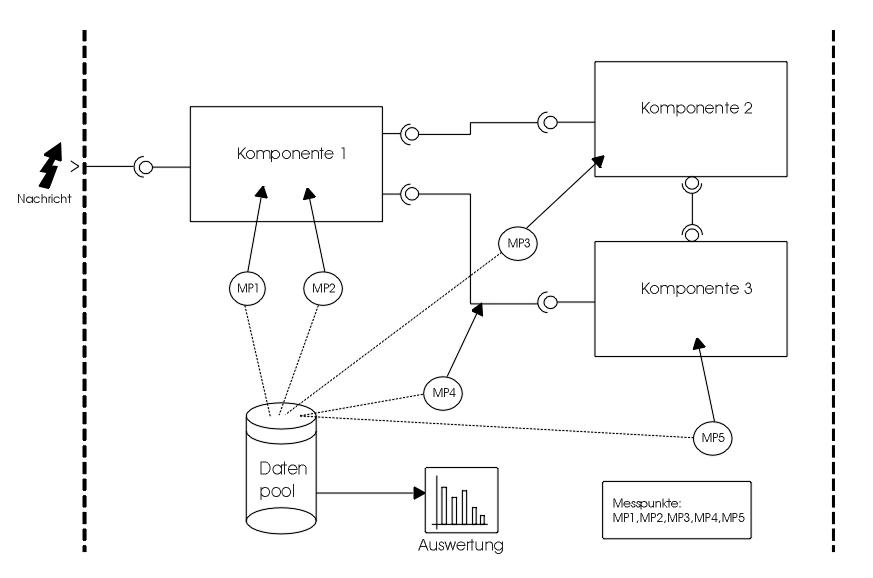
\includegraphics[width=13cm]{../res/simul.jpg}}
\caption{Schematische Darstellung der Simulation}
\label{pic:simul}
\end{center}
\end{figure}

\subsection{Ziele des Individuellen Projektes}
\label{sec:einleitung:ziele}
Ziel dieses Projektes ist die Erstellung einer Infrastruktur f�r die in Abschnitt \ref{sec:einleitung:motivation} erl�uterte Simulation in Form eines Frameworks. Bestandteil des Frameworks wird die Modellierung des Systems und der Komponenten, ein Modell zur Simulation von Anfragen an Dienste des Systems und die Auswertung der gesammelten Daten sein. Diese Bestandteile werden in einer Simulationsumgebung gekapselt.
\par
Bei der Entwicklung wird verst�rkt darauf geachtet, dass kleinere �nderungen und Erweiterungen des Frameworks nicht gro�e �nderungen der Implementierung zur Folge haben. So ist es beispielsweise w�nschenswert, dass einige sich von Modell zu Modell h�ufig �ndernde Bestandteile austauschen lassen, ohne eine Zeile Quellcode des Frameworks �ndern zu m�ssen. Weiterhin sollen Entwurfsentscheidungen, die die Umsetzung einer neuen Modellierung verhindern, �nderbar sein. Das bedeutet, dass die Bestandteile des Frameworks unabh�ngig voneinander austauschbar sein m�ssen.
\par
Das Projekt gliedert sich in die drei im Proposal \cite{lit:proposal} angegebenen Entwicklungsinkremente. Am Ende jedes Inkrementes wird ein der Entwicklungsstufe angepasster Prototyp entstehen, welcher das Framework in seinem aktuellen Stand benutzt.

\subsection{Aufbau dieser Ausarbeitung}
\label{sec:einleitung:aufbau}

Die Ausarbeitung gliedert sich in drei inhaltliche Teile, welche von dieser Einleitung und einem abschlie�enden Fazit eingeschlossen sind.
\par
Der erste Teil befasst sich mit der Kl�rung theoretischer Fragen in Bezug auf die Modellierung von Komponentenarchitekturen und der Simulation. Hierzu werden anf�nglich einige Grundlagen zur Modellierung von Komponenten erarbeitet, welche als Ziel das Modell der gesamten Komponentenarchitektur haben. Darauf aufbauend werden in diesem Modell potentielle Zeitverbraucher identifiziert. Der letzte Teil dieses Kapitels stellt das f�r das Framework entwickelte Simulationsmodell vor.
\par
Der zweite und gleichzeitig gr��te Teil dieser Ausarbeitung ist dem Entwurf des Frameworks gewidmet. Dieser beginnt mit dem Festlegen einiger allgemeiner Anforderungen an das Framework. Der zweite Teil dieses Kapitels erarbeitet eine sinnvolle Architektur des Frameworks. Das bedeutet, dass an dieser Stelle das Framework in seine groben Bestandteile gegliedert wird. Innerhalb dieser Teile werden dann unter Betrachtung von speziellen an den jeweiligen Teil gestellten Anforderungen einzelne Komponenten identifiziert. Der dritte Teil des Entwurfs bildet dann schlie�lich die Architektur mit ihren Komponenten auf Klassen und Pakete ab. Hier werden einige der Entwurfsentscheidungen zum besseren Verst�ndnis des Frameworks detailiert erkl�rt.
\par
Das dritte und abschlie�ende inhaltliche Kapitel der Ausarbeitung geht auf die Anwendung des Frameworks ein. Hierzu wird anhand eines Beispiels die Benutzung der Basisfunktionalit�t beschrieben. Weiterhin wird auf die Erweiterungsm�glichkeiten und deren Ansatzpunkte im Framework eingegangen. Um den Umfang der Funktionalit�t des Frameworks einsch�tzen zu k�nnen, wird dem Leser abschlie�end ein �berblick �ber die Grenzen des Frameworks vermittelt.  % Einleitung

%% ++++++++++++++++++++++++++++++++++++++++++
%% Anhang
%% ++++++++++++++++++++++++++++++++++++++++++

\appendix
%\include{anhang_a}
%\include{anhang_b}

%% ++++++++++++++++++++++++++++++++++++++++++
%% Literatur
%% ++++++++++++++++++++++++++++++++++++++++++
%  mit dem Befehl \nocite werden auch nicht 
%  zitierte Referenzen abgedruckt
\cleardoublepage
\phantomsection
\addcontentsline{toc}{chapter}{\bibname}
\nocite{*} 
\bibliographystyle{itmalpha}
\bibliography{diplarb}
%% ++++++++++++++++++++++++++++++++++++++++++
%% Index
%% ++++++++++++++++++++++++++++++++++++++++++
\ifnotdraft{
\cleardoublepage
\phantomsection
\addcontentsline{toc}{chapter}{Index}
\printindex            % Index, Stichwortverzeichnis
}
\end{document}
%% end of file